\documentclass[10pt]{article}
\usepackage[a4paper,margin=25mm]{geometry}
\usepackage[T1]{fontenc}
\usepackage{lmodern}
\usepackage{amssymb}
\usepackage{microtype}
\usepackage{graphicx}
\usepackage{booktabs}
\usepackage{tabularx}
\usepackage{longtable}
\usepackage{array}
\usepackage[table]{xcolor}
\usepackage{tikz}
\usetikzlibrary{arrows.meta,positioning,shapes.geometric}
\usepackage[round,authoryear]{natbib}
\usepackage{hyperref}
\hypersetup{colorlinks=true,linkcolor=blue!55!black,citecolor=blue!55!black,urlcolor=blue!55!black,pdftitle={Auditing Temporal and Identity Dependence in SCONE-bench}}
\newcommand{\dataset}{SCONE-bench}
\newcommand{\ncase}{417}
\newcommand{\statusbox}{\fcolorbox{orange!70!black}{orange!8}{\parbox{0.94\linewidth}{\textbf{Accountability notice.} This is a mechanically checked draft, not a submission-ready manuscript. The draft author and public repository authority are identified; final affiliations, CRediT roles, declarations, downstream reuse rights, independent scientific reproduction, and submission approval remain open.}}}
\setlength{\emergencystretch}{2em}

\title{Auditing Temporal and Identity Dependence in \dataset:\\Dual-Provider Historical State Reconstruction of 417 Smart-Contract Incidents}
\author{Zubaer Mahmood Zubraj\\\small Draft author; final affiliation and CRediT metadata pending}
\date{Draft generated 29 August 2026}

\begin{document}
\maketitle
\statusbox

\begin{abstract}
\textbf{Context:} Historical smart-contract benchmarks are often counted by incident rows, although a row's usable pre-incident history and independence depend on deployment time, code reuse, and proxy architecture. \textbf{Objective:} We audit these dependencies in the current 417-case \dataset{} cohort without evaluating a detector or making population-level vulnerability claims. \textbf{Method:} We reuse closed historical envelopes whose upstream evidence records verified status, a strict snapshot closure, block-hash-pinned reads, and two provider families. For each case, we measure whether the contract existed 1 hour, 24 hours, 7 days, and 30 days before its incident; compare chain--address, address-only, exact-runtime, and metadata-stripped runtime identities; and count specified ERC-1967 implementation/beacon and ERC-1167 indicators. \textbf{Results:} All 417 cases existed at least 24 hours before their incident, 352 (84.4\%, Wilson 95\% interval 80.6--87.6\%) existed at 7 days, and 275 (65.9\%, 61.3--70.3\%) existed at 30 days. Address identity assigns 14 rows to duplicate groups, versus 46 under exact runtime and 56 after metadata stripping. Sixty-seven cases (16.1\%, 12.9--19.9\%) expose at least one specified proxy indicator. \textbf{Conclusion:} Evaluation capacity and effective independence in this cohort vary with the temporal landmark and identity abstraction. The audit provides a reproducible cohort profile and boundary conditions, not evidence of detector accuracy, causal risk, or prevalence beyond \dataset.
\end{abstract}

\noindent\textbf{Keywords:} smart contracts; benchmark validity; historical state; code reuse; proxy contracts; reproducibility

\section{Introduction}
Smart-contract security evaluation increasingly uses curated datasets and executable historical incidents. Frameworks such as SmartBugs standardize static-analysis execution \citep{diangelo2023smartbugs}; SC-Bench provides a large audit-oriented corpus \citep{xia2025scbench}; EVMbench and later reevaluations expose the sensitivity of agent conclusions to task construction, scaffolds, and possible contamination \citep{wang2026evmbench,peng2026reevaluating}. CyberChainBench extends historical-fork evaluation across chains \citep{huang2026cyberchainbench}. These resources make previously difficult experiments possible, but a benchmark's nominal row count is not automatically its number of temporally usable or independent evaluation units.

The current \dataset{} repository contains 417 historical incidents \citep{scone2026}. An earlier report described a 405-case snapshot and local historical forks \citep{anthropic2025smartcontracts}. We treat the newer 417-case cohort as a finite benchmark population and ask three deliberately narrow questions:
\begin{enumerate}
  \item At which pre-incident landmarks did each benchmark contract already exist?
  \item How does effective dependence change across address- and bytecode-based identity abstractions?
  \item How many rows expose a specified, observable proxy-linkage indicator?
\end{enumerate}
Our contribution is the joint audit and its reproducible artifacts. The temporal test itself, hashing, metadata stripping, and proxy standards are established mechanisms; we make no ``first'' claim. The useful negative result is equally important: the audit cannot establish detector performance, vulnerability prevalence, causal risk, or real-world effectiveness.

\section{Related work and strongest prior art}
Dataset validity is already a central concern in smart-contract research. DIVE explicitly reports lifecycle-specific features and duplicate removal \citep{alsunaidi2026dive}; prior empirical work finds extensive source/function-level cloning in Ethereum contracts \citep{khan2023cloning}. These studies motivate identity sensitivity but do not answer it for \dataset's incident rows. EIP-1898 standardizes block-hash selectors for canonical historical reads \citep{eip1898}; ERC-1967 defines proxy implementation, beacon, and admin slots \citep{erc1967}; ERC-1167 defines recognizable minimal-proxy runtime code \citep{erc1167}. Table~\ref{tab:priorart} records the bounded prior-art comparison used to avoid overstating novelty.

\begin{table*}[t]
\centering\small
\caption{Strongest-prior-art matrix. ``Not located'' means not found within the documented search scope, not universal absence.}
\label{tab:priorart}
\begin{tabularx}{\textwidth}{>{\raggedright\arraybackslash}p{2.5cm}XXXXX}
\toprule
Work & Historical incidents & Historical state & Identity audit & Temporal audit & Proxy audit \\
\midrule
\dataset{} & Yes & Fork block & Not located & Not located & Not located \\
Re-evaluating EVMbench & Yes & Evaluation dependent & Contamination focus & No & No \\
CyberChain-\allowbreak Bench & Yes & Historical forks & Not located & Not located & Proxy subset for patching \\
DIVE & No & Lifecycle features & Duplicates removed & No & Not central \\
This audit & 417 rows & Dual-provider, block-hash-pinned upstream evidence & Four abstractions & 1h/24h/7d/30d & Specified observable indicators \\
\bottomrule
\end{tabularx}
\end{table*}

\section{Materials and methods}
\subsection{Frozen cohort and evidence gate}
The unit of analysis is one of the 417 case envelopes in the frozen local snapshot. The analysis fails closed unless every envelope is marked \texttt{VERIFIED}, has \texttt{strict\_snapshot\_closed=true}, and records both Alchemy and Infura provider families. It reuses upstream deployment time, incident time, runtime bytecode, and normalized proxy fields. The source tree is read-only; all derivatives are written to an isolated MPP directory.

The cohort contains 226 BSC, 181 Ethereum, 9 Base, and 1 Arbitrum cases (Table~\ref{tab:cohort}). This is a benchmark census, not a probability sample of deployed contracts.

\begin{table}[h]
\centering
\caption{Cohort composition (T3).}
\label{tab:cohort}
\begin{tabular}{lrr}
\toprule Chain & Cases & Percent \\
\midrule BSC & 226 & 54.2 \\
Ethereum & 181 & 43.4 \\
Base & 9 & 2.2 \\
Arbitrum & 1 & 0.2 \\
\bottomrule
\end{tabular}
\end{table}

\subsection{Estimands}
For case $i$, let $d_i$ be deployment time and $t_i$ incident time. Landmark eligibility is $E_{i,\ell}=\mathbb{1}[t_i-d_i\geq\ell]$ for $\ell\in\{1\mathrm{h},24\mathrm{h},7\mathrm{d},30\mathrm{d}\}$. This definition was frozen after an integration test detected and corrected an early implementation that had incorrectly substituted snapshot-cutoff lead for deployment age. The correction and its timing are preserved in the deviation record.

Four identity keys are compared: chain--address, address only, SHA-256 of exact runtime bytecode, and SHA-256 after removing a recognized Solidity CBOR metadata trailer. Each identity reports unique keys, groups of size at least two, rows in such groups, maximum group size, cross-address groups, and cross-chain groups. Equality defines a fingerprint family only.

Observable proxy linkage is the union of non-null ERC-1967 implementation, non-null ERC-1967 beacon, and recognized ERC-1167 target fields. The admin slot is reported separately because it does not identify a delegate target by itself. This deliberately incomplete rule produces a lower-bound indicator count.

\subsection{Statistical and reproducibility plan}
Because the frozen cohort is fully enumerated, the primary estimands are counts and proportions. Two-sided 95\% Wilson intervals are supplied as descriptive uncertainty aids. No hypothesis test, multiplicity adjustment, imputation, model fitting, or causal estimator is used. All computations use deterministic Python standard-library code, sorted output, fixed CSV schemas, and no network access or randomness. Algorithms~1--3 give the auditable logic.

\begin{figure*}[t]
\centering
\resizebox{\textwidth}{!}{%
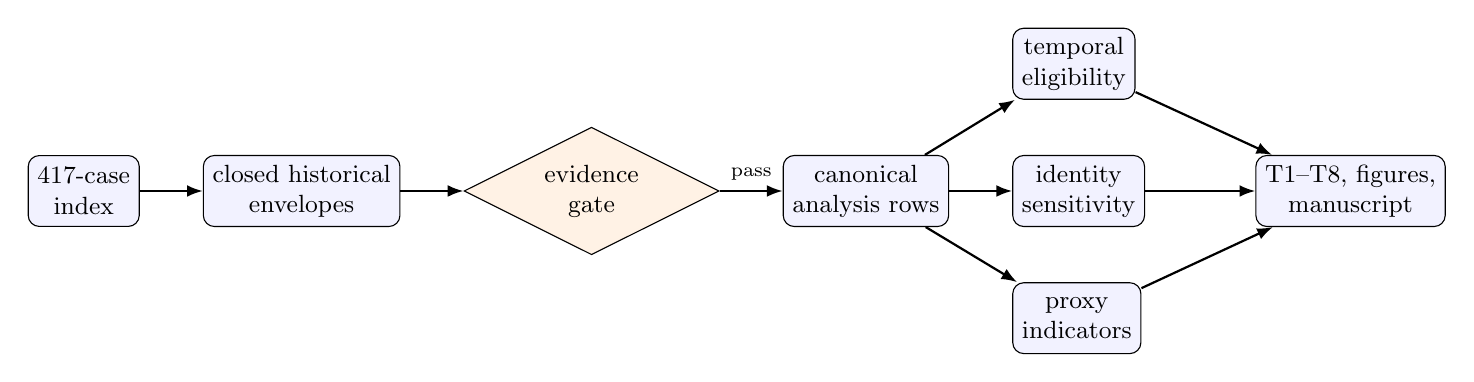
\begin{tikzpicture}[node distance=7mm and 8mm, every node/.style={font=\small}, box/.style={draw,rounded corners,align=center,minimum height=9mm,fill=blue!5}, gate/.style={draw,diamond,aspect=2,align=center,fill=orange!10}, arr/.style={-{Latex[length=2mm]},thick}]
\node[box] (index) {417-case\\index};
\node[box,right=of index] (env) {closed historical\\envelopes};
\node[gate,right=of env] (gate) {evidence\\gate};
\node[box,right=of gate] (rows) {canonical\\analysis rows};
\node[box,above right=of rows] (temp) {temporal\\eligibility};
\node[box,right=of rows] (ident) {identity\\sensitivity};
\node[box,below right=of rows] (proxy) {proxy\\indicators};
\node[box,right=14mm of ident] (paper) {T1--T8, figures,\\manuscript};
\draw[arr] (index)--(env); \draw[arr] (env)--(gate); \draw[arr] (gate)--node[above,font=\scriptsize]{pass}(rows);
\draw[arr] (rows)--(temp); \draw[arr] (rows)--(ident); \draw[arr] (rows)--(proxy);
\draw[arr] (temp)--(paper); \draw[arr] (ident)--(paper); \draw[arr] (proxy)--(paper);
\end{tikzpicture}
}
\caption{Analysis architecture. Arrows represent data flow, not causality. Editable Mermaid source is included with the artifact.}
\label{fig:architecture}
\end{figure*}

\begin{minipage}{0.96\linewidth}
\textbf{Algorithm 1: Temporal landmark eligibility.}
For each case $i$, parse deployment time $d_i$ and incident time $t_i$.
Fail closed if either value is absent or if $d_i>t_i$.
For each predeclared landmark $\ell\in\{1\mathrm{h},24\mathrm{h},7\mathrm{d},30\mathrm{d}\}$,
set $E_{i,\ell}=\mathbb{1}[t_i-d_i\geq\ell]$.
Report $\sum_i E_{i,\ell}/N$ with a two-sided 95\% Wilson interval.
The historical snapshot cutoff is audited separately and never substituted for deployment age.
\end{minipage}

\vspace{0.8em}
\begin{minipage}{0.96\linewidth}
\textbf{Algorithm 2: Identity sensitivity.}
For every case, construct four fingerprints: chain--address,
address only, SHA-256 of exact runtime bytecode, and SHA-256 of runtime bytecode
after removing the recognized Solidity CBOR metadata trailer.
Group equal fingerprints, count unique identities, groups of size at least two,
rows in those groups, cross-address groups, and cross-chain groups.
No bytecode equality result is interpreted as semantic equivalence.
\end{minipage}

\vspace{0.8em}
\begin{minipage}{0.96\linewidth}
\textbf{Algorithm 3: Observable proxy linkage.}
Normalize the upstream ERC-1967 implementation, admin, and beacon values and the
recognized ERC-1167 target. Count an implementation, beacon, or ERC-1167 target
as an observable proxy indicator; report admin separately because an admin slot
alone does not establish a proxy target. The resulting count is a lower bound,
not a complete proxy classifier.
\end{minipage}


\section{Results}
\subsection{Temporal eligibility}
All 417 contracts existed at both the 1-hour and 24-hour landmarks. At 7 days, 352 were eligible (84.4\%, Wilson 95\% interval 80.6--87.6\%); at 30 days, 275 were eligible (65.9\%, 61.3--70.3\%). Deployment-to-incident age ranged from 25.48 hours to 55,430.26 hours, with median 2,325.71 hours. Figure~\ref{fig:temporal} and Table~\ref{tab:primary} report the prespecified outcomes.

\begin{figure}[h]
\centering
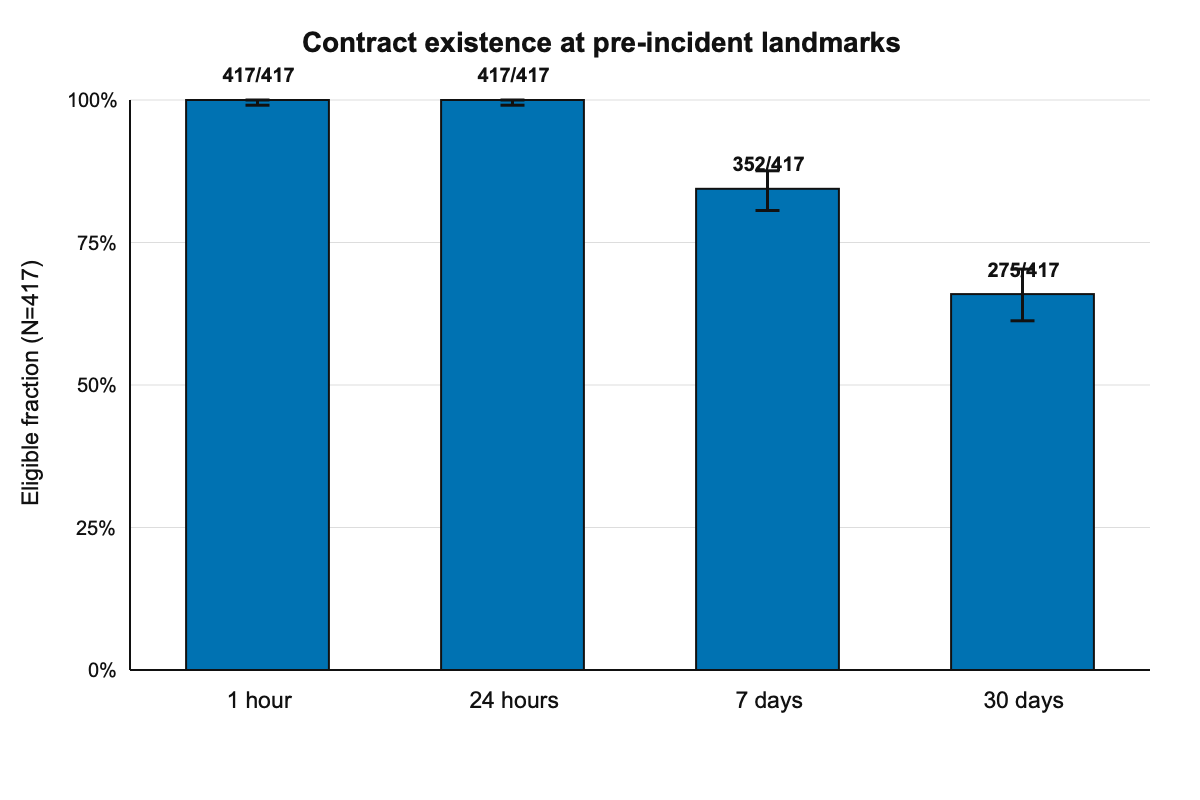
\includegraphics[width=\linewidth]{figure1-temporal-eligibility.png}
\caption{Contract existence at pre-incident landmarks. Error bars are two-sided 95\% Wilson intervals; counts use the fixed denominator $N=417$.}
\label{fig:temporal}
\end{figure}

\begin{table*}[t]
\centering\small
\caption{Primary temporal and proxy results (T4).}
\label{tab:primary}
\begin{tabular}{llrrrr}
\toprule Section & Metric & $n$ & $N$ & Percent & Wilson 95\% interval \\
\midrule
Temporal & 1 hour & 417 & 417 & 100.0 & 99.1--100.0 \\
Temporal & 24 hours & 417 & 417 & 100.0 & 99.1--100.0 \\
Temporal & 7 days & 352 & 417 & 84.4 & 80.6--87.6 \\
Temporal & 30 days & 275 & 417 & 65.9 & 61.3--70.3 \\
Proxy & implementation slot & 54 & 417 & 12.9 & 10.1--16.5 \\
Proxy & admin slot (separate) & 38 & 417 & 9.1 & 6.7--12.3 \\
Proxy & beacon slot & 1 & 417 & 0.2 & 0.0--1.3 \\
Proxy & ERC-1167 target & 12 & 417 & 2.9 & 1.7--5.0 \\
Proxy & any specified indicator & 67 & 417 & 16.1 & 12.9--19.9 \\
\bottomrule
\end{tabular}
\end{table*}

\begin{figure}[h]
\centering
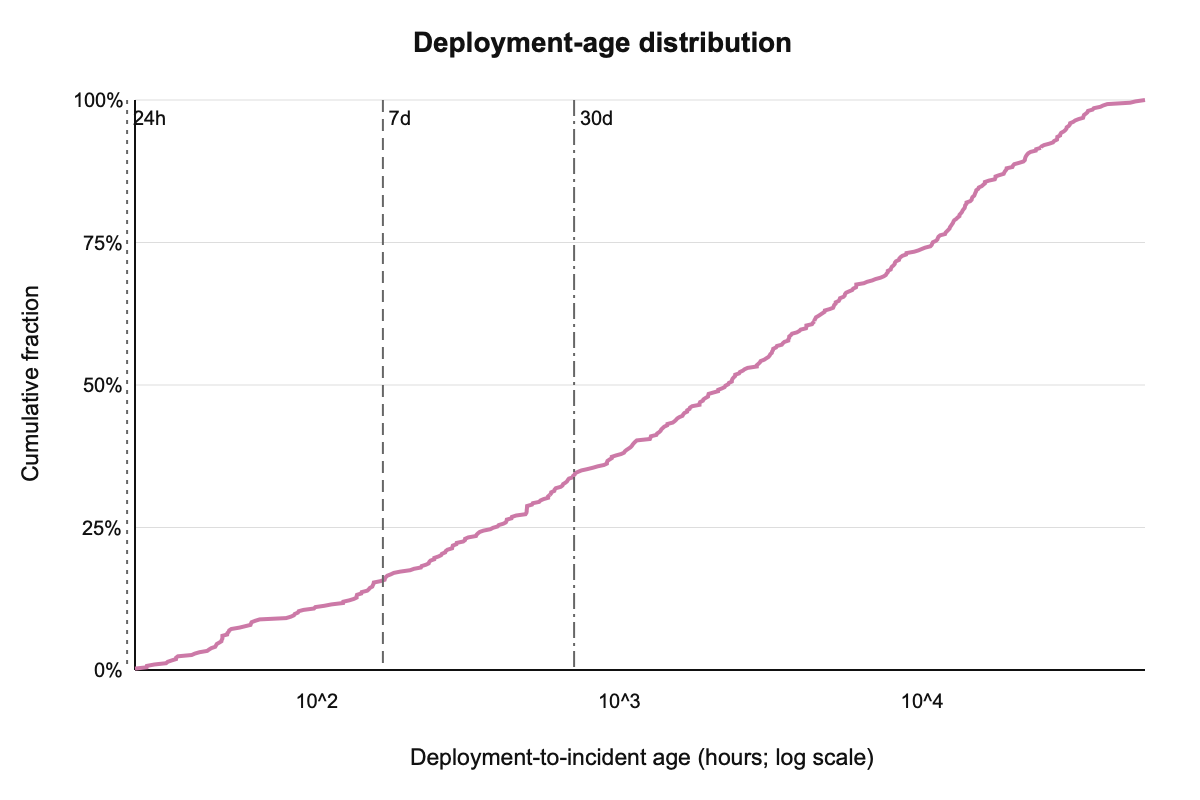
\includegraphics[width=\linewidth]{figure3-deployment-age-ecdf.png}
\caption{Empirical cumulative distribution of deployment-to-incident age on a logarithmic hour scale. Vertical lines mark 24 hours, 7 days, and 30 days.}
\label{fig:ecdf}
\end{figure}

\subsection{Identity sensitivity}
Chain--address and address-only keys each yield 410 unique identities, seven duplicate groups, and 14 rows in those groups. No additional cross-chain same-address collision appears in this cohort. Exact runtime bytecode yields 388 identities and 46 duplicate-group rows; ten of its 17 duplicate groups span addresses, and three groups (16 rows) span chains. Metadata stripping yields 382 identities and 56 duplicate-group rows; 14 of 21 groups span addresses and three groups (17 rows) span chains. The maximum runtime-family size is nine (Table~\ref{tab:identity}, Figure~\ref{fig:identity}).

\begin{table*}[t]
\centering\small
\caption{Identity-abstraction mechanism audit (T5).}
\label{tab:identity}
\resizebox{\textwidth}{!}{%
\begin{tabular}{lrrrrrr}
\toprule Identity & Unique & Groups & Rows & Cross-address groups & Cross-chain groups & Max size \\
\midrule
Chain--address & 410 & 7 & 14 & 0 & 0 & 2 \\
Address only & 410 & 7 & 14 & 0 & 0 & 2 \\
Exact runtime & 388 & 17 & 46 & 10 & 3 & 9 \\
Metadata-stripped runtime & 382 & 21 & 56 & 14 & 3 & 9 \\
\bottomrule
\end{tabular}
}
\end{table*}

\begin{figure*}[t]
\centering
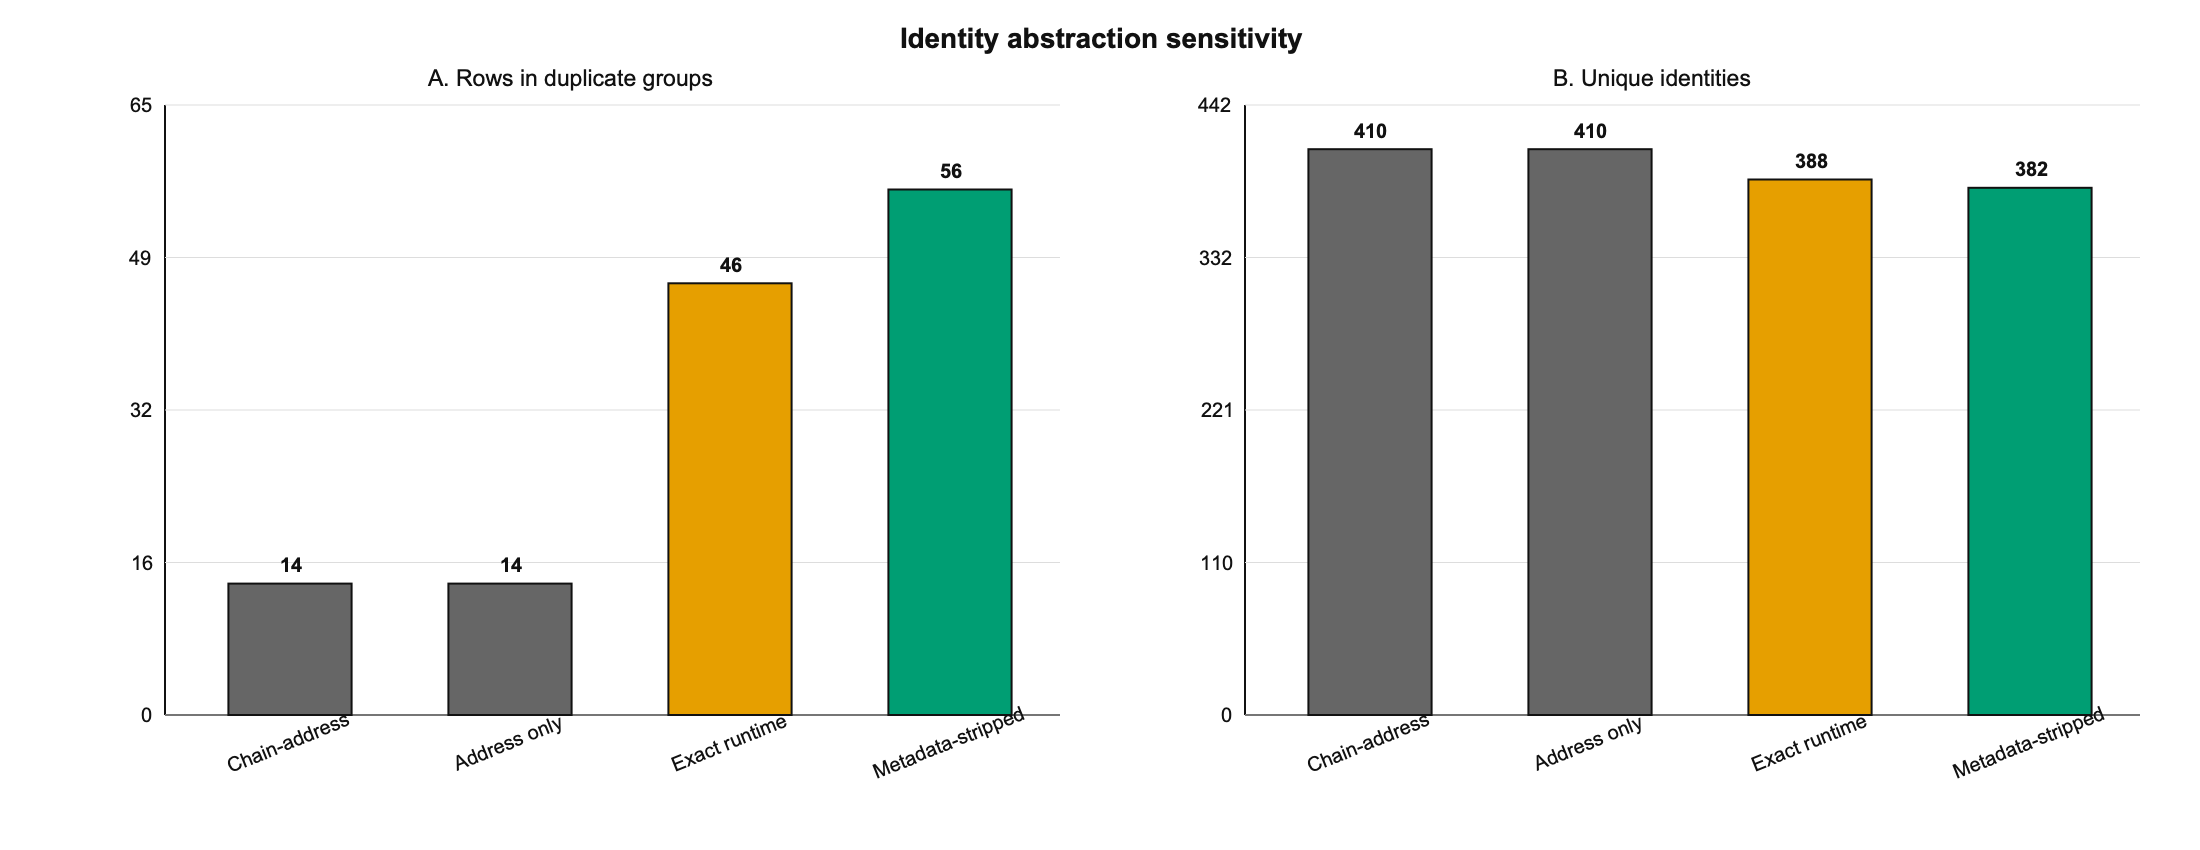
\includegraphics[width=\textwidth]{figure2-identity-sensitivity.png}
\caption{Sensitivity to the identity abstraction. Direct labels make the result interpretable without color.}
\label{fig:identity}
\end{figure*}

\subsection{Observable proxy linkage}
Fifty-four cases carry a non-null implementation slot, one a non-null beacon slot, and 12 a recognized ERC-1167 target. Their union contains 67 cases (16.1\%, Wilson 12.9--19.9\%). Thirty-eight admin-slot observations are reported separately. Overlap means component counts cannot be summed. The result is a cohort-specific lower bound under the declared indicator rule.

\section{Robustness and boundary analyses}
Metadata stripping adds ten duplicate-group rows and ten cross-address duplicate rows relative to exact runtime identity; it adds one cross-chain row. This demonstrates that an apparently small preprocessing choice changes the effective dependence estimate. Conversely, chain--address and address-only results coincide in this cohort. These are abstraction-sensitivity results, not proof that one identity is universally correct.

The temporal denominator is also landmark-dependent. A study requiring a 30-day pre-incident window has 275 eligible units before any additional exclusion, not 417. A study requiring only 24 hours retains all rows. This paper does not evaluate whether a particular downstream task actually needs each landmark.

\begin{table}[h]
\centering\small
\caption{Robustness and boundary comparisons (T6).}
\begin{tabularx}{\linewidth}{>{\raggedright\arraybackslash}p{3.0cm}rrX}
\toprule Comparison & Baseline & Alternative & Difference and boundary \\
\midrule
Address duplicate rows & 14 & 14 & 0; no added cross-chain address collision \\
Exact vs stripped duplicate rows & 46 & 56 & +10; metadata changes identity \\
Exact vs stripped cross-address rows & 32 & 42 & +10; semantic near-clones still excluded \\
Exact vs stripped cross-chain rows & 16 & 17 & +1; state/configuration may still differ \\
\bottomrule
\end{tabularx}
\end{table}

\section{Discussion}
The main implication is operational: a historical incident benchmark should publish a landmark-conditioned denominator and at least one dependence sensitivity analysis. A single nominal row count hides both. The results do not imply that 30 days is preferable to 7 days, nor that metadata-stripped bytecode is the definitive unit. They show how those choices alter the usable cohort.

Proxy architecture creates an additional linkage layer. The 67-case lower-bound indicator count signals that contract address alone can obscure implementation reuse or indirection. Future work could resolve implementation graphs at each landmark, identify semantic clone families, and test how cluster-aware resampling changes detector or agent uncertainty. Those are new studies, not results of this audit.

\subsection{Threats to validity}
\textbf{Construct validity.} Deployment and incident timestamps, bytecode, and proxy fields are reused from upstream envelopes. Exact bytecode is not semantic behavior, and the proxy rule omits nonstandard and diamond-style patterns. \textbf{Internal validity.} The script validates declared closure fields but does not independently recreate every upstream provider response. Correlated upstream or provider errors may remain. \textbf{External validity.} \dataset{} is a curated incident benchmark, not a probability sample; no percentage generalizes to all contracts, chains, vulnerabilities, or incidents. \textbf{Conclusion validity.} Wilson intervals are descriptive aids for a fixed cohort, not a basis for population inference. \textbf{Novelty validity.} The documented search found related benchmark-validity, lifecycle, and clone studies; no independent search challenger has certified the remaining differentiator.

\section{Reproducibility, ethics, and responsible use}
The bundle includes a row-level provenance manifest, input manifest, analysis code, tests, result CSV/JSON files, editable T1--T8 tables, SVG masters, PNG derivatives, Mermaid diagram sources, LaTeX source, BibTeX, and mechanical QA outputs. No participant recruitment, intervention, private key use, or new chain scraping occurs. The analysis processes public smart-contract incident metadata, but downstream row-level redistribution rights require human/legal review before public release. Security-sensitive details are not expanded beyond the upstream benchmark. The study makes no exploit-generation or operational safety claim.

Generative AI assisted planning, code generation, drafting, and internal checking under human direction. It is not an author, scientific verifier, or accountable submitter. A human author must validate every result, disclosure, citation, and source-rights statement before submission.

\section{Conclusion}
Within the current 417-case \dataset{} cohort, all contracts support a 24-hour pre-incident landmark, while 352 support 7 days and 275 support 30 days. Dependence rises from 14 duplicate-group rows under address identities to 46 under exact runtime and 56 after metadata stripping. Sixty-seven cases expose at least one specified proxy indicator. These findings support reporting landmark-conditioned and identity-conditioned benchmark denominators. They do not establish detector performance, causal vulnerability risk, or ecosystem prevalence. The artifact is mechanically reproducible locally; independent reproduction and accountable human approval remain prerequisites to upload.

\section*{Statements and Declarations}
\textbf{Funding:} Pending accountable-author confirmation.\\
\textbf{Competing interests:} Pending accountable-author confirmation.\\
\textbf{Ethics approval and consent:} No human or animal participants and no intervention; final institutional determination, if required, is pending accountable-author confirmation.\\
\textbf{Data availability:} The current \dataset{} repository is publicly accessible. Redistribution of this paper's row-level derivatives is pending source-rights review; aggregate tables and code are prepared in the local bundle.\\
\textbf{Code availability:} Analysis code and tests are prepared in the local reproducibility bundle; public repository/DOI pending author approval.\\
\textbf{Author contributions:} Zubaer Mahmood Zubraj is the named draft author and repository owner; final CRediT roles and any additional eligible authors require accountable confirmation.\\
\textbf{AI-use disclosure:} Generative AI assisted planning, code generation, drafting, and internal checking. Human authors must take responsibility for the final work.

\bibliographystyle{plainnat}
{\small\bibliography{references}}

\clearpage
\appendix
\section{Minimum artifact table set}
\begin{table}[h]
\centering\footnotesize
\caption{Proposed audit versus simpler baselines (T2).}
\begin{tabularx}{\linewidth}{lXXXX}
\toprule Approach & Temporal & Identity & Proxy & Main failure \\
\midrule
Row count & No & No & No & Overstates usable independent units \\
Address dedup & No & Address & No & Misses cross-address families \\
Exact runtime & No & Exact code & Partial & Metadata and proxy layers remain \\
This audit & Four landmarks & Four abstractions & Specified indicators & Still a lower bound \\
\bottomrule
\end{tabularx}
\end{table}

\begin{table}[h]
\centering\small
\caption{Feasibility and authority gates (T7).}
\begin{tabularx}{\linewidth}{l l X X}
\toprule Dimension & Status & Evidence & Remaining gate \\
\midrule
New collection & N/A & Read-only 417-case reuse & None \\
Determinism & Verified mechanically & Standard-library tests & Independent reproduction \\
Rights & At risk & SCONE Apache-2.0 & Row-level release review \\
Scientific independence & Blocked & Root produced/self-reviewed & Qualified independent reviewer \\
Submission authority & Blocked & Author/declarations unresolved & Accountable human approval \\
\bottomrule
\end{tabularx}
\end{table}

\begin{table}[h]
\centering\small
\caption{Negative findings and scope controls (T8).}
\begin{tabularx}{\linewidth}{X X}
\toprule Finding & Effect on claim \\
\midrule
No controls or detector evaluation & Cohort-validity audit only \\
Proxy rule incomplete & 67 is a lower-bound indicator count \\
Bytecode equality is not semantics & Groups are fingerprint families only \\
Cohort is not a probability sample & No ecosystem generalization \\
Novelty not independently certified & Submission remains gated \\
\bottomrule
\end{tabularx}
\end{table}

\section{Execution timeline}
\begin{center}
\resizebox{\textwidth}{!}{%
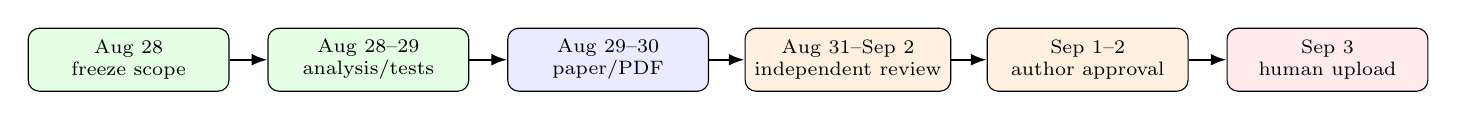
\begin{tikzpicture}[x=1.45cm,y=0.85cm, every node/.style={font=\scriptsize}, phase/.style={draw,rounded corners,minimum width=2.55cm,minimum height=8mm,align=center}, arr/.style={-{Latex[length=2mm]},thick}]
\node[phase,fill=green!10] (p1) at (0,0) {Aug 28\\freeze scope};
\node[phase,fill=green!10] (p2) at (2.1,0) {Aug 28--29\\analysis/tests};
\node[phase,fill=blue!8] (p3) at (4.2,0) {Aug 29--30\\paper/PDF};
\node[phase,fill=orange!12] (p4) at (6.3,0) {Aug 31--Sep 2\\independent review};
\node[phase,fill=orange!12] (p5) at (8.4,0) {Sep 1--2\\author approval};
\node[phase,fill=red!8] (p6) at (10.5,0) {Sep 3\\human upload};
\draw[arr] (p1)--(p2); \draw[arr] (p2)--(p3); \draw[arr] (p3)--(p4); \draw[arr] (p4)--(p5); \draw[arr] (p5)--(p6);
\end{tikzpicture}
}
\end{center}
The dates after local paper/PDF completion are targets, not completed scientific or authority gates.

\end{document}
